\title{4-bit binary counter.}
\date{}
\author{
	\IEEEauthorblockN{Daniel Josué Rodríguez Agraz}
	\IEEEauthorblockA{
		\textit{Communications and Electronics Enginnering, Unniversidad de Guadalajara}\\
	}
}

\documentclass[conference]{IEEEtran}
\def\endthebibliography{%
	\def\@noitemerr{\@latex@warning{Empty `thebibliography' environment}}%
	\endlist
}
\usepackage{filecontents,lipsum}
\usepackage[noadjust]{cite}
\usepackage{graphicx}
\usepackage{footmisc}
\usepackage{listings}
\usepackage{subcaption}
\usepackage{fancyhdr}
\usepackage{url}
\usepackage{hyperref}
\usepackage{array}
\usepackage{float}
\usepackage{adjustbox}
\usepackage{subcaption}
\hypersetup{
	colorlinks=true,
	linkcolor=black,
	urlcolor=blue,
	citecolor=black
}

\begin{document}
	
	\maketitle
	\begin{abstract}
		This document presents the design and verification process of a 4-bit binary counter digital circuit. The design and verification were conducted using the SystemVerilog hardware description language, with simulation and compilation performed in Questasim software. The implementation for the design was done using a state machine approach. Additionally, a test bench was developed to verify each instance and the final design, demonstrating the successful implementation of the circuit.
	\end{abstract}
	
	\section{Objectives}	
	\begin{itemize}
		\item Use Verilog to design and simulate a 4-bit binary counter.
		\item Implement a finite state machine for circuit design.
		\item Design a test bench for the circuit verification.
	\end{itemize}
	
	\section{Introduction}
	A counter is a digital circuit responsible of counting electronic events, such as pulses, by progressing through a sequence of binary states.
	An $n$-bit binary counter is made of n flip-flops and is able to count to up to $2^{n}-1$.
	We can divide digital counters into two main categories; synchronous and asynchronous \cite{floyd_fundamentos_nodate}.
	
	\subsection{Asynchronous Counter}
	An asynchronous counter is a digital counter where the internal flip-flops are connected in a cascade configuration. In this arrangement, the clock input for each flip-flop is derived from the output of the previous flip-flop, rather than all flip-flops sharing the same clock signal. This results in a ripple effect, where the change in state propagates through the flip-flops with some delay, which can limit the speed of the counter \cite{floyd_fundamentos_nodate}.
	
	
	\begin{figure}[H]
		\centering
		\includegraphics[width=0.7\columnwidth]{"Files/Diagrama en blanco - Página 1"}
		\caption{2 bit asynchronous counter.}
		\label{fig:diagrama-en-blanco---pagina-1}
	\end{figure}
	
	\vspace*{2cm}
	
	\subsection{Synchronous Counter}
	The synchronous digital counter has all of its flip-flops receiving the same clock signal simultaneously.  Since there is no ripple or propagation delay between the flip-flops, this type of counter is significantly faster than an asynchronous counter \cite{floyd_fundamentos_nodate}.
	
	\begin{figure}[H]
		\centering
		\includegraphics[width=0.7\columnwidth]{"Files/asinc count"}
		\caption{2 bit synchronous counter.}
		\label{fig:asinc-count}
	\end{figure}
	
    
	
	
	
	\section{Methodology}
	This project was developed using the SystemVerilog hardware description language, with Questasim software used for compilation and simulation. The project began with the definition of the counter's inputs and outputs, which are represented in Figure \ref{fig:diagram}. The counter features a preset value, which sets the starting point of the count and the value to which the counter returns after completing a full cycle. In addition to the preset, a reset input was implemented to restart both the count and the preset value.
	
	\begin{figure}[H]
		\centering
		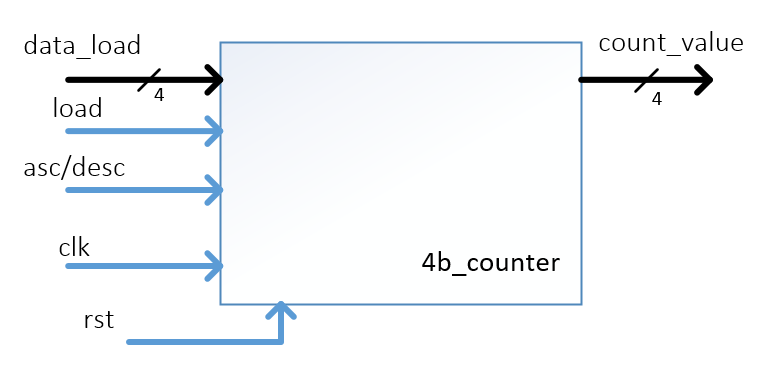
\includegraphics[width=0.7\columnwidth]{Files/Diagram}
		\caption{Representation of a 4-bit binary counter.}
		\label{fig:diagram}
	\end{figure}
	
	
	Figure \ref{fig:state_diagram} illustrates the flow diagrams for the state machine implemented in the counter. Two separate state machines were used for this implementation, as shown in the state diagram: one state machine manages the ascending count, while the other handles the descending count. The transitions between these states are governed by control variables, which determine whether the counter switches between counting up or down.
	\begin{figure}[H]
		\begin{subfigure}[b]{\columnwidth}
			\centering
			\includegraphics[width=\columnwidth]{"Files/Flow_chart asc"}
			\caption{State diagram for ascending cases.}
			\label{fig:flowchart-asc}
		\end{subfigure}
		\vspace*{1cm}
		\begin{subfigure}[b]{\columnwidth}
			\centering
			\includegraphics[width=\columnwidth]{"Files/Flow_chart asc"}
			\caption{State diagram for descending cases.}
			\label{fig:flowchart-desc}
		\end{subfigure}
		\begin{subfigure}[b]{\columnwidth}
			\centering
			\includegraphics[width=0.5\columnwidth]{"Files/Preset Flow chart"}
			\caption{State diagram for LOAD signal.}
			\label{fig:preset-flow-chart}
		\end{subfigure}
		
		
		\caption{State diagrams for 4-bit digital counter.}
		\label{fig:state_diagram}
	\end{figure}
	
	Below the implementation in verilog of the 4-bit digital counter is shown.
	
	\begin{lstlisting}[language=Verilog, 
		caption={2 bit full adder code hardware description in verilog.}, 
		label={code:FA_2B_Code}]
module Counter_4B(
  input reg [3:0] D_in,
  input wire LOAD, ASC_DESC,
  input wire clk, rst,
  output reg [3:0] COUNT
);

reg [3:0] D;
reg [3:0] next_state, present_state;

assign COUNT = present_state;

localparam [3:0]  s0 = 4'h0,
                  s1 = 4'h1,
                     .
                     .
                     .
                  s15 = 4'hF;

always @(posedge clk or posedge rst) 
begin
  if (rst) 
  begin
    present_state <= 'h0;
  end 
  else if (~LOAD) 
  begin
    D <= D_in;
    present_state <=D;
  end 
  else 
  begin
    present_state <= next_state;
  end
end

always @(*)
begin
// Ascending
if (ASC_DESC) 
begin
  case (present_state)
	s0:  next_state <= s1;
	s1:  next_state <= s2;
	     .
	     .
	     .
	s15: next_state <= D;
	default: next_state <= D; // Default state
    endcase 
    end 
    else // Descending
    begin
    case (present_state)
        s0: next_state <= s15;
        s1: next_state <= D;
            .
            .
            .
        s15: next_state <= s14;
        default: next_state <= D;
  endcase
end
end
endmodule
	\end{lstlisting}
	
	
	\section{Results}
	For the verification process, we loaded several preset values, as shown in Table \ref{}, and applied a range of test cases to validate the counter's functionality. These test cases involved altering the states of the control signals, such as the reset, reload, ascending, and descending states. By manipulating these control values, we ensured that the counter behaved as expected under different conditions, including resetting to the preset value, counting up and down correctly, and reloading when necessary.
	
	In the Figures \ref{fig:descendingpreset0} and \ref{fig:descendingpreset02} , the value '0' is loaded as the preset, and the ascend signal is low, resulting in a descending output.
	\begin{figure}[H]
		\centering
		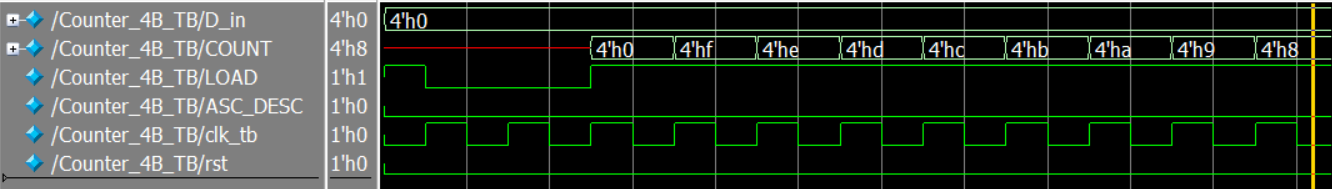
\includegraphics[width=\columnwidth]{descending_preset0}
		\caption{Simulation results for a '0' preset}
		\label{fig:descendingpreset0}
	\end{figure}
	
	\begin{figure}[H]
		\centering
		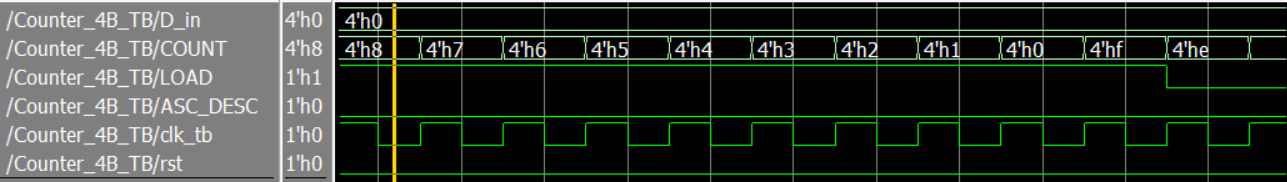
\includegraphics[width=\columnwidth]{descending_preset0_2}
		\caption{Simulation results for a '0' preset}
		\label{fig:descendingpreset02}
	\end{figure}
	
	To verify the correct operation of the reload function, a reload was performed. The result shows that the counter correctly returned to the preset value of '0', as shown in Figure \ref{fig:descendingpreset0wreload}, with the ascend signal still low, ensuring a descending output.
	
	\begin{figure}[H]
		\centering
		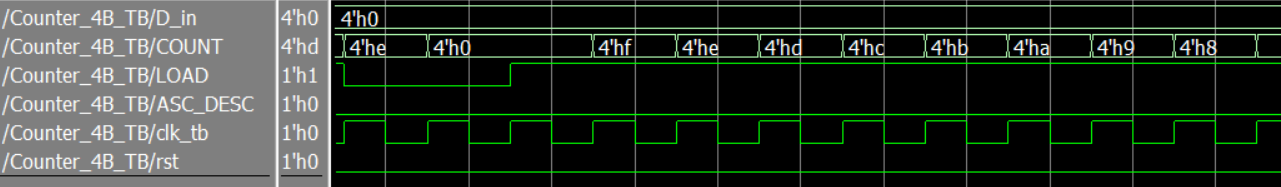
\includegraphics[width=\columnwidth]{descending_preset0_w_reload}
		\caption{Simulation results for a 0 preset and a reload of 0.}
		\label{fig:descendingpreset0wreload}
	\end{figure}
	
	Next, in Figure \ref{fig:descendingpreset7}, the preset value was set to '7', and the descend operation was verified.
	
	\begin{figure}[H]
		\centering
		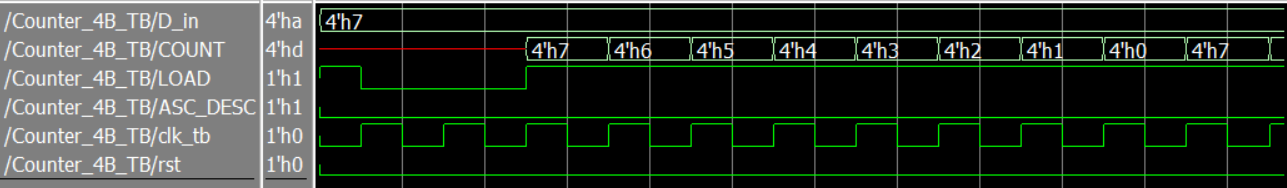
\includegraphics[width=\columnwidth]{descending_preset7}
		\caption{Simulation results for a 7 preset.}
		\label{fig:descendingpreset7}
	\end{figure}
	
	After loading a new value, a reload was conducted to ensure the counter correctly returns to the preset. Figure \ref{fig:descendingpreset7wreloada} shows the counter reloading a value of 'a' after the previous '7' preset, and a change to an ascending operation.
	
	\begin{figure}[H]
		\centering
		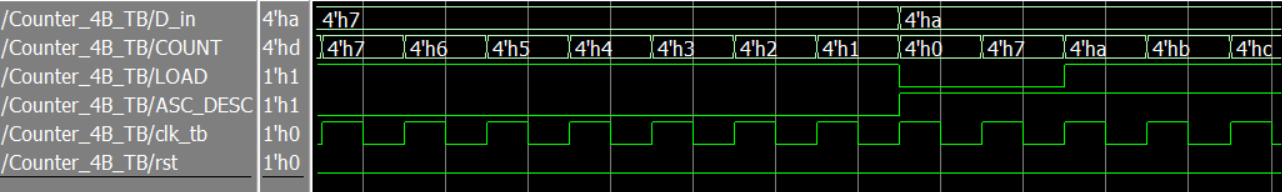
\includegraphics[width=\columnwidth]{descending_preset7_w_reload_a}
		\caption{Simulation results for a 7 preset and a reload of a value a.}
		\label{fig:descendingpreset7wreloada}
	\end{figure}
	
	In Figures \ref{fig:ascendingpreseta1reset} and \ref{fig:ascendingpreseta1reset1}, the counter was tested with an ascending count, with a preset value of 'a' and the reset signal active, verifying the counter's ability to start correctly after a reset.
	
	\begin{figure}[H]
		\centering
		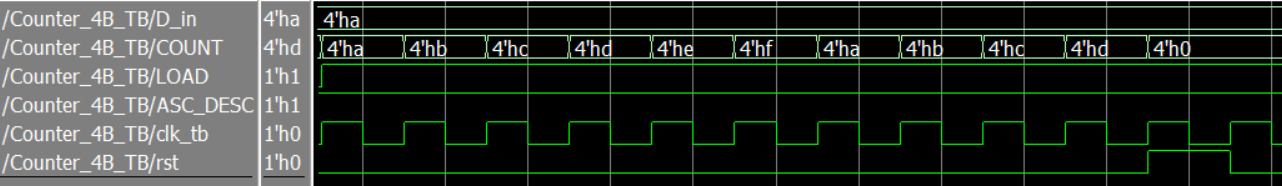
\includegraphics[width=\columnwidth]{ascending_preseta1_reset}
		\caption{Simulation results for an ascending count with an 'a' value preset, and a reset signal}
		\label{fig:ascendingpreseta1reset}
	\end{figure}
	
	\begin{figure}[H]
		\centering
		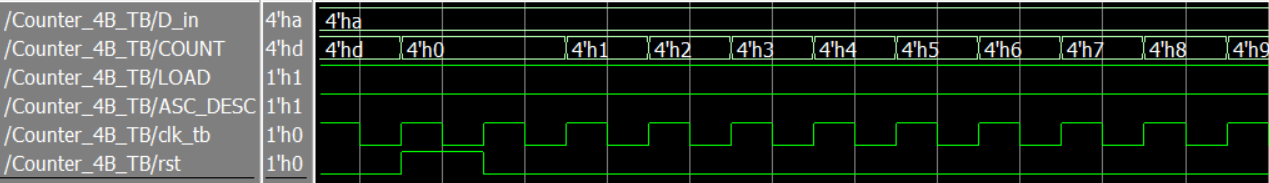
\includegraphics[width=\columnwidth]{ascending_preseta1_reset1}
		\caption{Simulation results for an ascending count with an 'a' value preset, and a reset signal.}
		\label{fig:ascendingpreseta1reset1}
	\end{figure}
	
	Lastly, after the reset, a reload was performed with the preset value of 'a'. The simulation results are presented in Figure \ref{fig:ascendingpreseta1reset2reloada}, confirming the correct operation of the reload and reset functions.
	
	\begin{figure}[H]
		\centering
		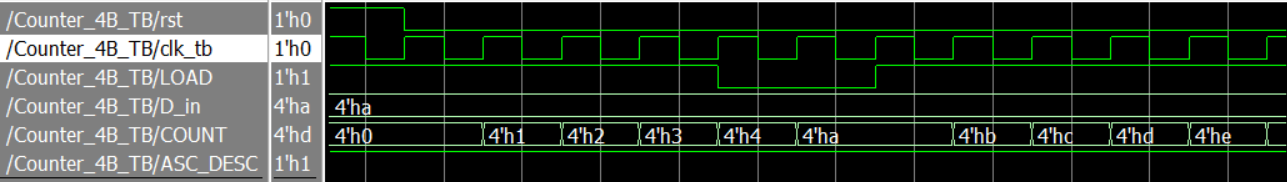
\includegraphics[width=\columnwidth]{ascending_preseta1_reset2_reloada}
		\caption{Simulation results for an ascending count with an 'a' value preset, and a reset signal.}
		\label{fig:ascendingpreseta1reset2reloada}
	\end{figure}
	
	\section{Conclusions}
	n this project, we successfully designed and implemented a 4-bit binary counter using the SystemVerilog hardware description language. The design utilized two state machines to manage both ascending and descending counts, and included a preset and reset functionality to provide flexibility and control over the counting process. The entire design was thoroughly verified through simulations in Questasim, ensuring correct operation under various conditions.
	This approach, combined with the implementation of a testbench, demonstrated the effectiveness of the design.
	
	
	
	
	\bibliographystyle{IEEEtran}
	\bibliography{References}
	
	
	
	
	
	
\end{document}
